% ---
% Capitulo de revisão de literatura
% ---


\chapter{Referencial Teórico}\label{ch:referencial_teorico}


\section{Autenticação e Identidade}\label{sec:autenticacaoeidentidade}
O problema de estabelecer uma associação entre um indivíduo e uma identidade pode ser dividido em duas categorias: autenticação e identificação~\cite{magalhaes2003biometria}.

\subsection{Autenticação}\label{subsec:autenticacao}
É o processo que verifica a autenticidade de um usuário, processo ou dispositivo.
Essa verificação confirma a legitimidade da entidade em questão.
Durante a autenticação, a parte que examina assegura que a entidade sendo verificada é genuína, e esta última participa ativamente na troca de informações~\cite{usmonov2021identification}.


Para~\cite{conti2017biometric} existem três tipos de autenticação\label{tipos-autenticacao}:

\begin{itemize}
    \item \textbf{Baseada em conhecimento:} utiliza informações que a pessoa sabe, como uma senha.
    \item \textbf{Com base em algo que a pessoa possua}, como um \textit{token} ou cartão inteligente.
    \item \textbf{Com base em características físicas da pessoa}, também conhecidas como biometria.
\end{itemize}


\section{Biometria}\label{sec:biometria}
O termo \("\)biometria\("\) vem das palavras gregas \("\)bios\("\) (vida) e \("\)metrikos\("\) (medida)~\cite{magalhaes2003biometria}.
É o estudo que visa identificar um indivíduo com base em suas características fisiológicas e comportamentais~\cite{handa2019comparative}, ou seja, biometria é uma forma de identificar pessoas usando características físicas ou comportamentais únicas.

Dos tipos mencionados em~\ref{tipos-autenticacao}, a biometria é tida como a abordagem mais segura, já que os atributos físicos de uma pessoa não podem ser furtados, cedidos ou esquecidos.
Falsear a autenticação biométrica é complicado e inviável, uma vez que avalia características singulares do indivíduo~\cite{dos2019tecnologias}.

\subsection{Tecnologias Biométricas}\label{subsec:biometria-tecnologias}

\subsubsection{Reconhecimento facial}\label{subsubsec:reconhecimento-facial}
É uma tecnologia capaz de identificar uma pessoa a partir de uma imagem digital ou de um vídeo, de modo que é comparado as características faciais selecionadas de uma determinada imagem com os rostos existentes numa base de dados~\cite{orvalho2019reconhecimento}.
Essas características incluem a distância entre os olhos, largura do nariz, posição das maçãs do rosto, linha da mandíbula, queixo, entre outras~\cite{adeoye2010survey}.
%O rosto não possui tantos traços únicos mensuráveis quanto impressões digitais ou íris dos olhos, o que faz com que a confiabilidade do reconhecimento facial seja levemente inferior a desses outros métodos biométricos.
%
%No entanto, ainda é adequado para muitas aplicações, especialmente pela sua conveniência para o usuário.
%O reconhecimento facial também pode ser utilizado em conjunto com o reconhecimento de impressões digitais ou outro método biométrico para desenvolver aplicações com necessidades de segurança mais críticas

%\begin{longtable}[c]{|l|l|}
    \hline
    \multicolumn{1}{|c|}{\textbf{Problemas}} & \multicolumn{1}{c|}{\textbf{Reconhecimento Facial}} \\ \hline
    \endfirsthead
    \endhead
    Sensor & \begin{tabular}[c]{@{}l@{}}
                 Resolução espacial, taxa\\ de quadros, distância da\\ câmera.
    \end{tabular} \\ \hline
    Envelhecimento & \begin{tabular}[c]{@{}l@{}}
                         Mudanças geométricas\\ entre a infância e a\\ adolescência, rugas e\\ flacidez facial.
    \end{tabular} \\ \hline
    Interação com o usuário & Poses e expressões. \\ \hline
    \begin{tabular}[c]{@{}l@{}}
        Mudanças no meio\\ ambiente
    \end{tabular} & \begin{tabular}[c]{@{}l@{}}
                        iluminação e cena de\\ fundo.
    \end{tabular} \\ \hline
    Outros fatores & \begin{tabular}[c]{@{}l@{}}
                         Maquiagem, acessórios,\\ e oclusão
    \end{tabular} \\ \hline
    \caption*{Fonte: Adaptado de~\cite{usmonov2021identification}}
\end{longtable}


\subsubsection{Impressão Digital}\label{subsubsec:geometria-mao}
A biometria de impressões digitais é um método de identificação individual baseado nas características únicas das papilas dérmicas presentes nas pontas dos dedos.
Essas características, conhecidas como minúcias, incluem padrões de cristas e sulcos exclusivos para cada pessoa, formados durante o desenvolvimento embrionário.
A tecnologia de identificação por impressão digital utiliza algoritmos para comparar as minúcias de uma amostra com as registradas em um banco de dados~\cite{de2020biometria}.

\subsubsection{Íris}\label{subsubsec:iris}
A biometria de íris é uma técnica de identificação baseada nas características únicas e estáveis da íris, o músculo responsável pela cor dos olhos.
Apresentando padrões complexos que diferem entre indivíduos e até entre os olhos esquerdo e direito de uma mesma pessoa, a íris é escaneada usando câmeras sensíveis ao infravermelho.
As imagens capturadas são codificadas e armazenadas para comparações futuras~\cite{de2020biometria}.

Devido à íris estar protegida pela córnea, ela permanece intacta ao longo da vida, fazendo da biometria de íris uma das tecnologias mais seguras e confiáveis, com taxas de erro inferiores a 1\%~\cite{de2020biometria}.

\subsubsection{Retina}\label{subsubsec:retina}
A biometria de retina é considerada uma das formas mais seguras de identificação pessoal, fundamentada na análise do padrão vascular único e complexo da retina no fundo do olho.
Este padrão é estável e inalterado do nascimento até a morte, exceto em casos de algumas doenças oculares~\cite{de2020biometria}.

A imagem da retina é capturada usando luz infravermelha, e as características vasculares são mapeadas e armazenadas para identificação futura.
Devido à sua alta precisão e baixa taxa de falsos positivos, a biometria de retina é frequentemente utilizada em ambientes que requerem segurança extremamente alta, como instalações militares, nucleares e para transações bancárias de grande valor~\cite{de2020biometria}.


\section{Reconhecimento Facial}\label{sec:reconhecimento-facial}

\subsection{Reconhecimento Facial e LGPD}\label{subsec:lgpd}
Nesta seção, será explorado implicações da lei no que diz respeito ao uso de imagens de pessoas.
A Lei Geral de Proteção de Dados Pessoais (LGPD) estabelece diretrizes importantes para o tratamento de dados pessoais, incluindo imagens, com o objetivo de proteger os direitos fundamentais de liberdade e de privacidade.

\subsubsection{Lei nº 13.709}
A partir da Lei nº 13.709 de 2018\footnote{Lei nº 13.709 de 2018~\url{https://www.planalto.gov.br/ccivil_03/_ato2015-2018/2018/lei/l13709.htm}}, estabelece regras sobre o tratamento de dados pessoais, inclusive aqueles coletados por meio de imagens, com o objetivo de proteger a privacidade e a liberdade das pessoas físicas~\cite{brasil2018lgpd}.
A seguir estão alguns pontos-chave da lei sobre o uso de imagens de pessoas extraídos da lei:

\begin{itemize}
    \item \textbf{Consentimento do Titular:} O tratamento de dados pessoais (que podem incluir imagens) só poderá ocorrer mediante consentimento do titular, salvo em casos específicos previstos em lei, como o cumprimento de uma obrigação legal ou para a proteção da vida ou da incolumidade física do titular ou de terceiros (Art.\ 7º).

    \item \textbf{Finalidade, Idoneidade e Necessidade:} O tratamento dos dados deve ter finalidade legítima, específica e informada ao titular, sendo compatível com as finalidades informadas (Art.\ 6º).
    Além disso, deve limitar-se ao mínimo necessário para atingir os seus objetivos, evitando o tratamento excessivo de dados.

    \item \textbf{Direitos do Titular:} O titular dos dados tem o direito de obter informações claras sobre a coleta e utilização de seus dados, incluindo a finalidade específica do tratamento (Art.\ 9).
    Ele também tem o direito de solicitar a correção, eliminação ou anonimização de dados desnecessários, ou tratados em desconformidade com a LGPD (Art.\ 18).

    \item \textbf{Tratamento de Dados Sensíveis:} A LGPD categoriza determinados tipos de dados, como aqueles relativos à origem racial ou étnica, opiniões políticas, crenças religiosas ou filosóficas, ou dados sobre saúde, ou vida sexual, como sensíveis.
    O seu tratamento requer cuidados adicionais e, em muitos casos, o consentimento específico do titular (Art.\ 11).

    \item \textbf{Segurança e Sigilo:} Os controladores e operadores de dados devem adotar medidas de segurança para proteger os dados pessoais de acessos não autorizados e de situações acidentais ou ilícitas (Art.\ 46).

    \item \textbf{Responsabilidade e Prestação de Contas:} Os agentes de tratamento (controladores e operadores) devem demonstrar a adoção de medidas eficazes capazes de comprovar o cumprimento das normas de proteção de dados (Art.\ 6º).
\end{itemize}

\item
Em resumo, a LGPD exige que a utilização de imagens de pessoas como dados pessoais seja feita de forma responsável, transparente e com a devida proteção da privacidade, respeitando os direitos dos titulares desses dados.


\section{Localização Exterior - GPS}\label{sec:localizacao}
GPS é a sigla da abreviatura de \textit{Global Positioning System}, ou Sistema de Posicionamento Global em português~\cite{gpsdesigning}.
Também chamado de NAVSTAR-GPS (Sistema de Navegação por Satélites com Tempo e Distância), é um sistema de navegação por rádio criado pelo Departamento de Defesa dos EUA. Foi criado originalmente para a navegação militar americana~\cite{novais2014localizaccao}.

É o método de identificar a posição geográfica de um objeto, pessoa ou dispositivo eletrônico.
Para isso, utiliza-se de informações provenientes de sinais de~\hypertarget{receptores}{GPS, torres de celular, endereços \textit{IP} ou redes  \textit{Wi-Fi}}.
Em resumo, permite o rastreamento em tempo real da localização de uma entidade~\cite{da2019sistemas}.

O GPS consiste em uma constelação de 24 satélites que orbitam a Terra a uma altitude aproximada de 20.200 km acima do nível do mar.
Essa configuração permite que os~\hyperlink{receptores}{receptores} determinem sua posição em qualquer lugar do planeta com notável precisão~\cite{el2002introduction}.

\subsection{Localização Interna - (Indoor)}\label{subsec:localizacao-indoor}

É uma tecnologia projetada para localização em ambientes internos, como andares de prédios, tuneis, salas ou auditórios~\cite{mittelstadt2018bluepath}.
Um dos fatores que aumentam a confiabilidade da localização de uma pessoa ou objeto em um determinado local é o GPS, entretanto essa tecnologia apresenta melhor desempenho em ambientes abertos, tendo uma grande imprecisão em ambientes fechados.

Quando um receptor está em um espaço interno, torna-se muito difícil decodificar os sinais GPS, uma vez que eles são atenuados por edifícios e paredes.
Isso resulta em perda de potência do sinal e, consequentemente, em erros na localização do receptor.
Nesse contexto, existe a localização indoor~\cite{mittelstadt2018bluepath}.

\subsubsection{Tecnologias de Localização Indoor}\label{subsubsec:tecnologias-localizacao-indoor}
Conforme o entedimento de~\cite{novais2014localizaccao} em sua tese de mestrado \("\)Localização Indoor em Ambientes Inteligentes\("\), ele que explica que as tecnologias de localização indoor geralmente são sem fio, visando uma maior aceitação dos usuários, pois andar com cabos para se localizar em um ambiente não é conveniente.
Dessa forma, as tecnologias wireless proporcionam mais conforto, comodidade e segurança.
Há várias maneiras de prover a localização em ambientes internos, algumas serão explicadas a seguir conforme o autor.

\subsubsubsection{Wi-Fi}\label{subsubsubsec:wifi}
A Wi-Fi (Wireless Fidelity) foi estabelecida em 1999 pela Interbrand\footnote{\url{https://interbrand.com/}} para a Wi-Fi Alliance\footnote{\url{https://www.wi-fi.org/}}, que visa assegurar a compatibilidade entre dispositivos Wi-Fi. Utiliza a norma IEEE 802.11, com acréscimos como os padrões 802.11b/g/n/ac, e permite comunicação entre dispositivos por ondas de rádio acima de 2.4 GHz. Os pontos de acesso conectam vários dispositivos sem fio e podem comunicar entre si, com alcance de aproximadamente 35 metros em ambientes internos e 110 metros em externos.

A prevalência de redes Wi-Fi em locais públicos e privados facilitou sua adoção em sistemas de localização indoor.
Esses sistemas são específicos para cada edifício e podem guiar pessoas ou robôs com dispositivos móveis Wi-Fi. A precisão aumenta ao limitar as possíveis posições dos dispositivos e fornecer plantas dos locais para reduzir distorções de sinal.

Os sistemas de localização podem operar nos próprios dispositivos (localização implícita) ou em servidores (localização explícita).
A configuração envolve uma fase de treino, coletando intensidade do sinal Wi-Fi e identificadores SSID, e uma fase online que compara os dados recebidos com os mapas de rádio para determinar a posição do dispositivo via técnicas de localização determinísticas ou probabilísticas.

\subsubsubsection{ZigBee}\label{subsubsubsec:zigbee}
ZigBee é um conjunto de protocolos de comunicação de baixa taxa de dados para conexão sem fio de curto alcance, baseado no padrão \textit{IEEE 802.15.4} (É um padrão para redes sem fio de baixo consumo de energia e baixa velocidade de dados, usado em \textit{IoT}) e desenvolvido pela Connectivity Standards Alliance (CSA) \footnote{\url{https://csa-iot.org/}} (anteriormente conhecida como ZigBee Alliance), uma organização sem fins lucrativos.

A tecnologia é econômica e de baixo consumo energético, ideal para automação residencial e monitoramento, mas também é aplicável em localização indoor.
Funciona com rádio frequência e requer a posição conhecida de emissores no ambiente para localizar objetos ou dispositivos através da comunicação entre os emissores.

\subsubsubsection{RFID}\label{subsubsubsec:rfid}
A tecnologia RFID (Radio-Frequency Identification) é usada para armazenar e recuperar dados por meio de transmissão eletromagnética.
O RFID permite identificar e rastrear itens e foi precursor dos sistemas modernos ao identificar aviões amigos ou inimigos.
Um sistema RFID inclui leitores e etiquetas, que comunicam usando frequência de rádio.
Etiquetas passivas não têm bateria e refletem o sinal do leitor com informações moduladas, enquanto etiquetas ativas têm alcance maior, até 100 metros, e são mais rápidas, sendo lidas em menos de 100 milissegundos.

Para localização indoor, RFID é mais complexo, geralmente utilizando o dispositivo móvel como leitor e etiquetas distribuídas como pontos de referência para estimar a localização através do sinal de força recebido (RSSI), exigindo que o edifício seja dividido em zonas para essa finalidade.


\section{Tecnologias}\label{sec: tecnologias}

\subsection{Flutter}\label{subsec: flutter}
O Flutter é uma estrutura multiplataforma destinada ao desenvolvimento de aplicações móveis de alto desempenho.
Lançado publicamente em 2016 pela Google, ele se destaca por sua capacidade de executar aplicações não apenas em sistemas Android e iOS, mas também no Linux, macOS, Windows e Fuschia, o sistema operacional de próxima geração da Google, que o selecionou como seu framework no nível de aplicação~\cite{wu2018react}.

Conforme na Figura~\ref{fig:architecture} a particularidade do Flutter reside em sua abordagem de renderização: em vez de usar web views ou depender de widgets OEM do dispositivo, o Flutter utiliza seu próprio motor de renderização de alto desempenho para desenhar todos os componentes da interface do usuário.
Essa característica permite a criação de aplicações com desempenho comparável ao das aplicações nativas.
Em termos de arquitetura, o código do motor escrito em C/C++ é compilado com o NDK do Android e com LLVM no iOS, enquanto qualquer código Dart é compilado antecipadamente (AOT) em código nativo durante o processo de compilação~\cite{flutter}.

\begin{figure}[H]
    \centering
    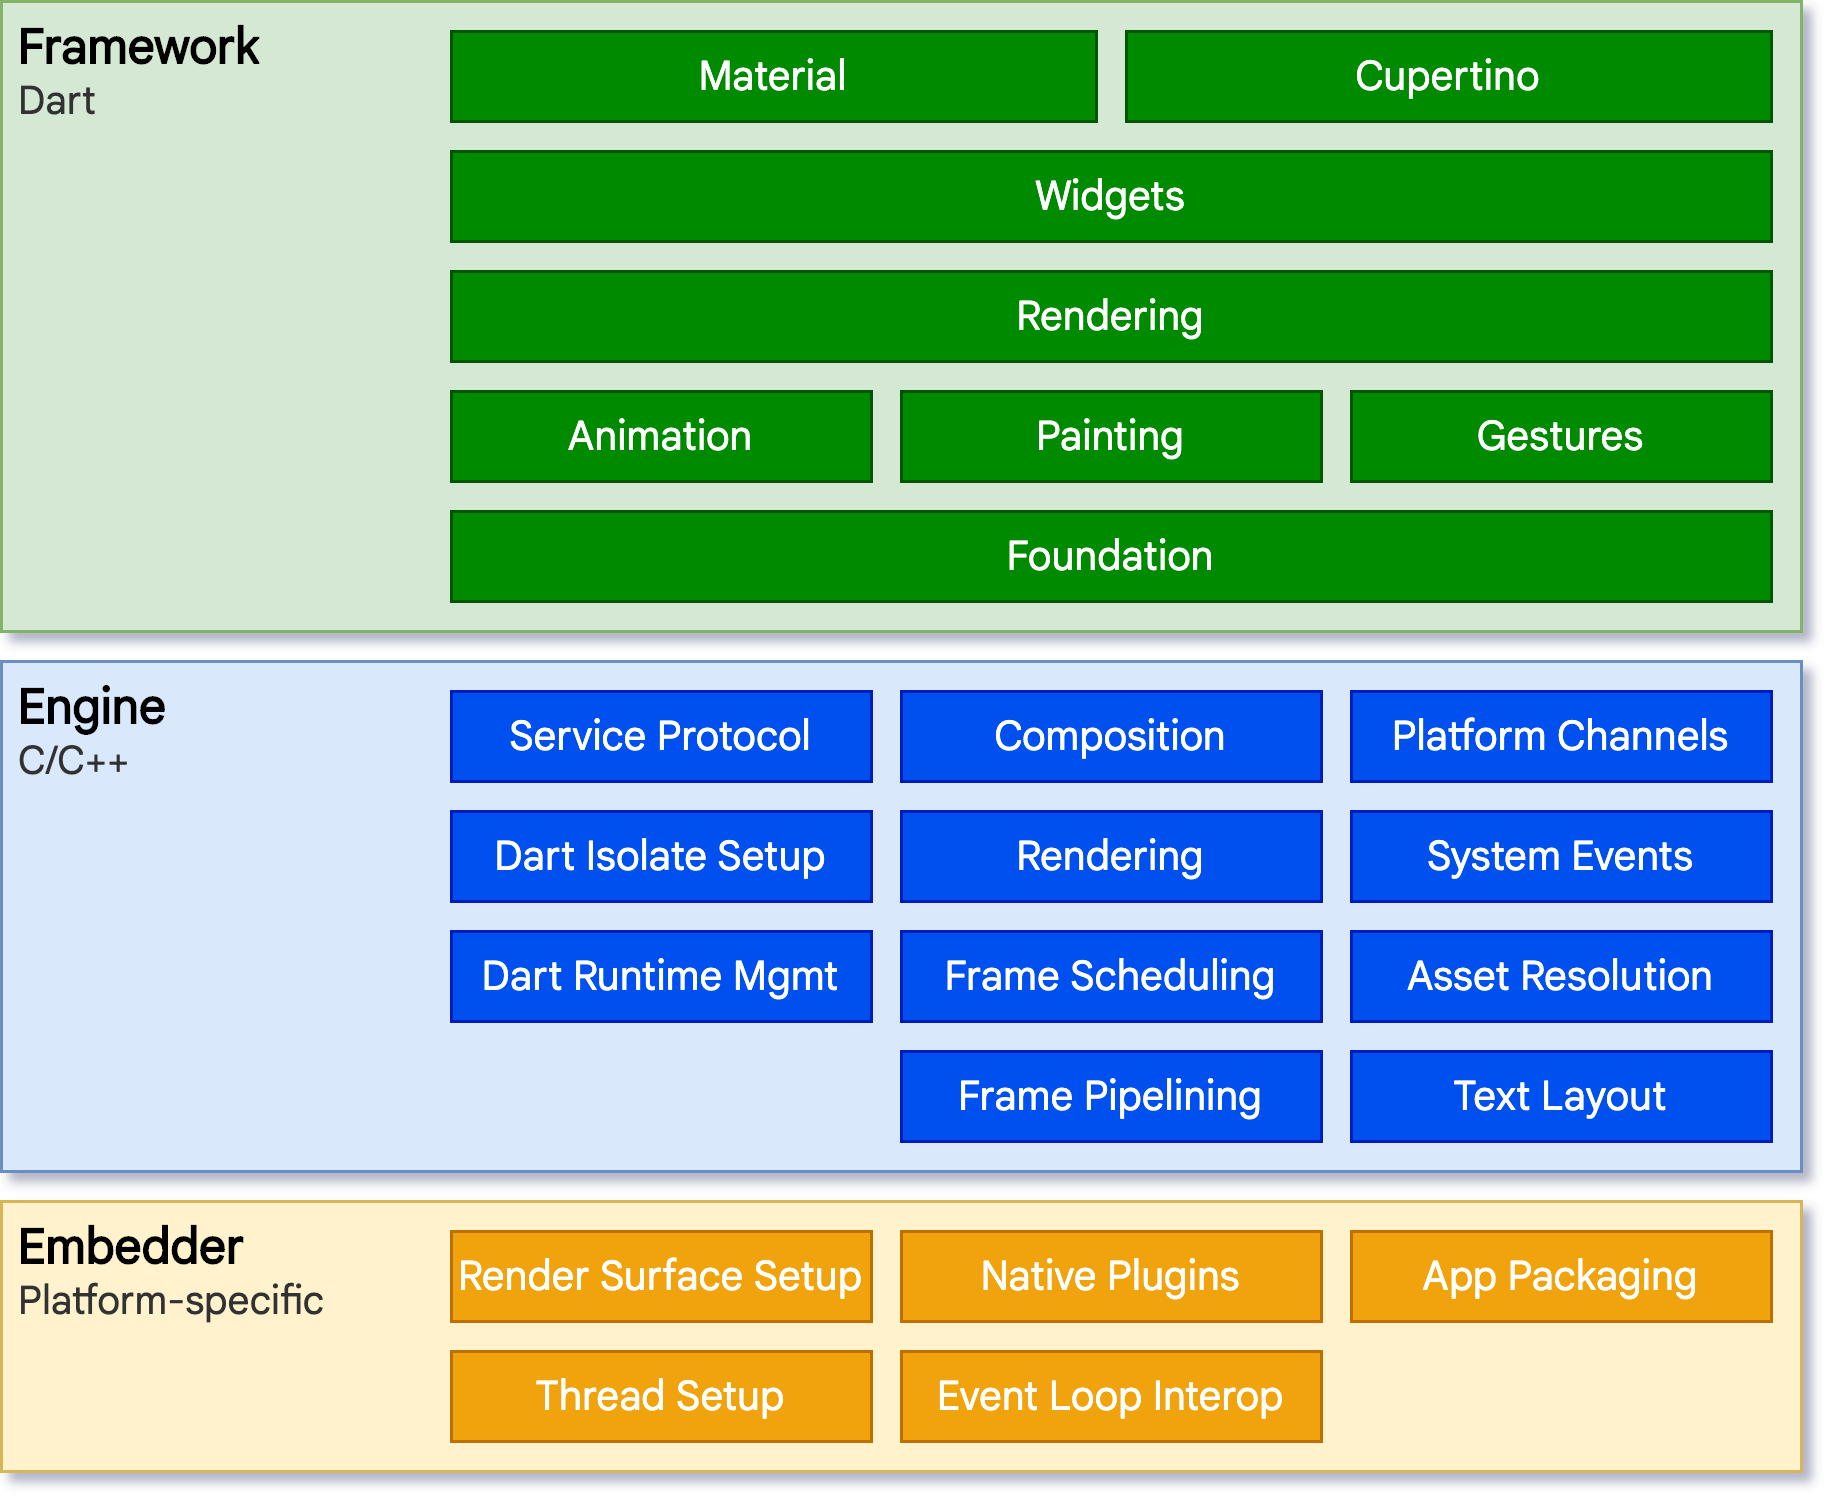
\includegraphics[width=0.7\textwidth]{imagens/flutter_architecture}
    \caption{Visão geral da arquitetura do Flutter~\cite{flutter}.}
    \label{fig:architecture}
\end{figure}

Além disso, o Flutter oferece suporte ao ~\textit{hot-reload} com estado (stateful hot-reload) durante o desenvolvimento, uma funcionalidade considerada fundamental para acelerar o ciclo de desenvolvimento~\cite{wu2018react}.
O ~\textit{hot-reload} com estado é implementado pela injeção de código-fonte atualizado na Dart VM em execução, sem alterar a estrutura interna da aplicação, o que significa que todas as transições e ações são preservadas após o hot-reloading~\cite{flutter}.

\subsection{Dart}\label{subsec: dart}
No Flutter, todas as aplicações são escritas utilizando a linguagem de programação Dart.
Dart é desenvolvida e mantida pela Google e tem sido amplamente usada dentro da própria empresa, demonstrando sua capacidade de desenvolver aplicações web em larga escala, como no AdWords.
A Dart foi originalmente criada para substituir e suceder o JavaScript, incorporando a maioria das características importantes da próxima norma do JavaScript (ES7), incluindo palavras-chave como “async” e “await”.
Para tornar a linguagem atraente também para desenvolvedores que não estão familiarizados com JavaScript, a Dart possui uma sintaxe semelhante à do Java.

Assim como outros sistemas que utilizam visualizações reativas, as aplicações Flutter atualizam a árvore de visualização a cada novo quadro (frame).
Esse comportamento resulta no desafio de gerar muitos objetos que podem existir apenas durante um único quadro.
Para lidar com isso, o Dart, como uma linguagem de programação moderna, está otimizada para gerenciar este cenário no nível da memória, com o auxílio do “Garbage Collection Geracional”.
Essa técnica de coleta de lixo ajuda a gerenciar a memória de forma eficiente, garantindo que os objetos de curta duração sejam coletados rapidamente, o que é crucial para manter o desempenho em um ambiente onde o estado da interface do usuário pode mudar rapidamente~\cite{flutter}.

\subsection{Widgets}\label{subsec: widgets}
Os Widgets são elementos centrais em uma aplicação Flutter, responsáveis por serem atraentes e funcionais, pois são a interface com a qual o usuário interage diretamente.
Eles não só controlam e afetam o comportamento das visualizações, mas também gerenciam e respondem às ações dos usuários~\cite{faust2020using}.
É fundamental que os Widgets sejam rápidos, tanto na renderização quanto na animação.

Diferentemente do React Native, que reutiliza os widgets OEM, a equipe do Flutter optou por fornecer seus próprios widgets.
Isso significa que o Flutter decide quando e como os widgets são renderizados, deslocando os widgets e o motor de renderização do sistema operacional para dentro da própria aplicação.
Esse método permite maior personalização e extensibilidade dos widgets.
No entanto, essa abordagem aumenta o tamanho da aplicação devido à inclusão do motor de renderização~\cite{flutter}.

\subsection{Quarkus}\label{subsec: quarkus}
~\cite{vsipek2020enhancing} descreve que Quarkus é um framework Java nativo para Kubernetes que foi projetado para otimizar aplicações javas tanto para a JVM quanto para o GraalVM, reduzindo o uso de memória e facilitando a criação de imagens nativas.
Oferece um ambiente de desenvolvimento que detecta automaticamente mudanças e atualiza a aplicação em tempo real, aumentando a produtividade do desenvolvedor.
Inclui o servidor web Undertow para melhor desempenho e suporta programação assíncrona e microserviços.
Quarkus prioriza segurança, permitindo extensões para práticas recomendadas e integração com provedores terceirizados para autenticação e gerenciamento de usuários.
Utiliza tecnologias estáveis como Hibernate ORM, Eclipse Vert.x, Netty e RestEasy, proporcionando uma configuração unificada e recarga rápida, sendo uma plataforma robusta para aplicações Java em ambientes serverless.







